\documentclass{beamer}
\usepackage[danish]{babel}
\usepackage[applemac]{inputenc}
\usepackage{beamerthemesplit}
\usepackage{graphics,epsfig, subfigure}
\usepackage{url}
\usepackage[UTF8]{inputenc}
\usepackage{multirow}
%\usepackage{movie15}
\usepackage[version=3]{mhchem}

\definecolor{kugreen}{RGB}{50,93,61}
\definecolor{kugreenlys}{RGB}{132,158,139}
\definecolor{kugreenlyslys}{RGB}{173,190,177}
\definecolor{kugreenlyslyslys}{RGB}{214,223,216}
\setbeamercovered{transparent}
\mode<presentation>{
\usetheme{Dresden}
 \usecolortheme[named=kugreen]{structure}
 \useinnertheme{circles}
 \usefonttheme[onlymath]{serif}
 \setbeamercovered{transparent}
 \setbeamertemplate{blocks}[rounded]
}
\setbeamertemplate{background}{\includegraphics[width=0.15\textwidth]{natlogo.jpg}}

\title{Cryogenic cavity optomechanics with ultrahigh-Q membrane resonators}
\subtitle{Supervisor: Eugene Polzik\\
Co-supervisor: Albert Schlie{\ss}er}
\author{Willi Carlsen}
\institute{Quantop \\Niels Bohr Institute \\University of Copenhagen}
\date{September 2015}
\begin{document}


\frame{\titlepage\vspace{-0.5cm}}

\section{Key points}

\frame{
\frametitle{Key points}
\begin{enumerate}
	\item{Introduction}
	\begin{itemize}
	\item{Cavity optomechanics}
	\item{Mechanical resonator}
	\end{itemize}
	\item{Setup}
	\item{Experimental results}
	\item{Conclusion and outlook}
	\item{Questions?}
\end{enumerate}
}


\section{Introduction}

\frame{
\frametitle{Introduction}
\begin{itemize}
\item Spying
\item Classically $T = 0$ K
\item Quantum mechanically $n_{\mathrm{phonon}} = 0$
\end{itemize}
\begin{center}
\includegraphics[scale=0.2]{spy.png}
\end{center}
\centering
\tiny{Credits: https://www.youtube.com/watch?v=pktWhH6m_DM}
}

\frame{
\frametitle{Sample}
\begin{itemize}
\item High-stress silicon nitride (\ce{Si3N4})
\item Macroscopic object
\item Put it in the ground state
\end{itemize}
\begin{center}
\includegraphics[scale=0.15]{Seidel_02.jpg}
\end{center}
}

\frame{
\frametitle{Introduction}
\begin{itemize}
\item Cavity ultra sensitive measurements
\item Sensitivity of femtometer ($10^{-15}$ m)
\item Cavity optomechanical model - mirror on a spring
\item Optical cooling
\end{itemize}
\begin{center}
\includegraphics[scale=0.21]{florian_opt.pdf}
\end{center}
\centering
\tiny{Credits: Ivan Favero and Florian Marquardt 2014 New J. Phys. 16 085006}
}

\section{Optomechanics}
\frame{
\frametitle{Model of cavity optomechanics}
%\begin{center}
%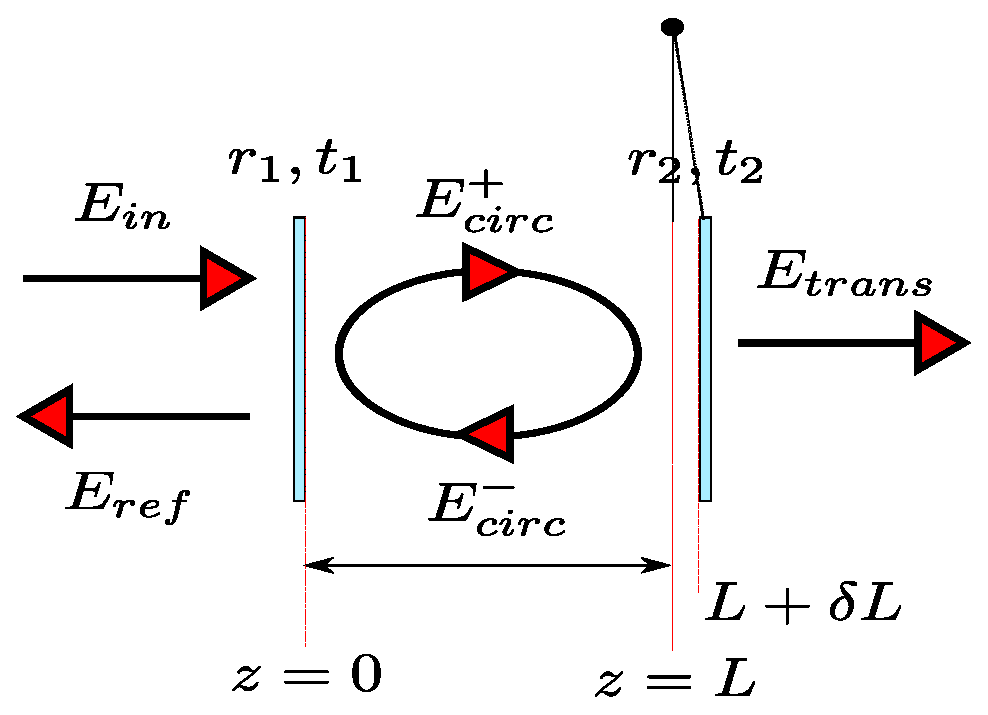
\includegraphics[scale=0.3]{E-field_model.eps}
%\end{center}
\begin{itemize}
\item Interaction Hamiltonian $\hat{H}_{int} = \hbar G\hat{x}\hat{a}^\dagger\hat{a}$
\item Coupling $G = \frac{\partial\omega_c}{\partial x}$
\item Radiation pressure force $F_{rad} = \frac{-\partial \hat{H}_{int}}{\partial \hat{x}}$
\end{itemize}
\begin{center}
\includegraphics[scale=1.5]{system.pdf}
\end{center}
}

\frame{
\frametitle{Sideband cooling}
\begin{itemize}
\item Scattering
\item Resolved sideband regime $\kappa \ll \Omega_m$
\end{itemize}
\begin{columns}
\begin{column}{0.3\textwidth}
\includegraphics[scale=0.25]{Stokes_anti-stokes_feynman.pdf}
\end{column}
\begin{column}{0.60\textwidth}
\includegraphics[scale=0.41]{resolved_sb.pdf}
\end{column}
\end{columns}
}

\frame{
\frametitle{Membrane-in-the-middle}
\begin{columns}
\begin{column}{0.45\textwidth}
\begin{equation*}
G = \frac{\partial\omega_c}{\partial x}
\end{equation*}
\includegraphics[scale=0.4]{transfer_matrix.png}
\end{column}
\begin{column}{0.45\textwidth}
\includegraphics[scale=0.3]{transfer_matrix_python.png}
\end{column}
\end{columns}
}

\section{Membrane}
\frame{
\frametitle{Mechanical resonator $\Gamma_m$}
\begin{columns}
\begin{column}{0.45\textwidth}
\includegraphics[scale=0.3]{rms.pdf}
\begin{equation*}
\langle x^2 \rangle = \frac{k_BT_{eff}}{\Omega_{m}^2m_{eff}} \propto n_{phonon}
\end{equation*}
\end{column}
\begin{column}{0.45\textwidth}
\includegraphics[scale=0.29]{modes.png}
\end{column}
\end{columns}
}

\section{Setup}
\frame{
\frametitle{Optical table setup}
\begin{itemize}
\item Pre-setup
\end{itemize}
\begin{center}
\includegraphics[scale=0.5]{setup.pdf}
\end{center}
}

\frame{
\frametitle{Optical table setup}
\begin{itemize}
\item Cryocavity setup
\end{itemize}
\begin{center}
\includegraphics[scale=0.5]{cryocavity.pdf}
\end{center}
}

\frame{
\frametitle{Sample}
\begin{itemize}
\item High-stress silicon nitride (\ce{Si3N4}) membrane sample
\item Thickness $\sim 45$ nm
\item Mechanical (3,3)-mode $\Omega_m/2\pi \sim 2.2$ MHz
\item Phononic bandgap
\end{itemize}
\begin{center}
\includegraphics[scale=0.15]{Seidel_02.jpg}
\end{center}
}

\section{Experiments}

\frame{
\frametitle{Mechanical ringdown $\Gamma_m$}
\begin{equation*}
Q = \frac{\Omega_m}{\Gamma_m}
\end{equation*}
\begin{center}
\includegraphics[scale=0.39]{ringdown_33_4k.pdf}
\end{center}
}

\frame{
\frametitle{Sample holder $T_{init}$}
\begin{columns}
\begin{column}{0.45\textwidth}
\begin{equation*}
T_{eff} = T_{init}\frac{\Gamma_m}{\Gamma_{eff}}
\end{equation*}
\includegraphics[scale=0.11]{bigBud_v09_new.png}
\end{column}
\begin{column}{0.45\textwidth}
\includegraphics[scale=0.5]{mim_setup.pdf}
\end{column}
\end{columns}
}


\frame{
\frametitle{Coupling point $G$}
\begin{columns}
\begin{column}{0.10\textwidth}
\includegraphics[scale=0.6]{2kz_bubble_with_mem.pdf}
\end{column}
\begin{column}{0.80\textwidth}
\includegraphics[scale=0.45]{2kz_mod.pdf}
\end{column}
\end{columns}
}

\frame{
\frametitle{Detuning $\bar{\Delta}$ and cavity linewidth $\kappa$}
\begin{itemize}
\item Optomechanically induced transparency
\end{itemize}
\begin{columns}
\begin{column}{0.45\textwidth}
\includegraphics[scale=0.318]{omit_fit_detuning_new.pdf}
\end{column}
\begin{column}{0.45\textwidth}
\includegraphics[scale=0.4]{OMIT_probes_cavity.pdf}
\end{column}
\end{columns}
}

\frame{
\frametitle{Detuning $\bar{\Delta}$ and cavity linewidth $\kappa$}
\begin{itemize}
\item Optomechanically induced transparency
\end{itemize}
\begin{columns}
\begin{column}{0.45\textwidth}
\includegraphics[scale=0.318]{omit_fit_detuning_new.pdf}
\end{column}
\begin{column}{0.45\textwidth}
\includegraphics[scale=0.3]{detuning_vs_DC.pdf}
\end{column}
\end{columns}
}

\frame{
\frametitle{Single photon coupling $g_0$}
\begin{columns}
\begin{column}{0.45\textwidth}
\begin{equation*}
\Gamma_{eff}(g, \bar{\Delta}, \kappa)
\end{equation*}
\includegraphics[scale=0.305]{omit_fit_dip_zoom.pdf}
\end{column}
\begin{column}{0.45\textwidth}
\begin{equation*}
g = g_0\sqrt{\bar{n}_{cav}}
\end{equation*}
\includegraphics[scale=0.3]{omit_g0.pdf}
\end{column}
\end{columns}
}

\frame{
\frametitle{Spectra of membrane $T_{eff}$}
\begin{center}
\includegraphics[scale=0.3]{cal_spec_newest0.pdf}
\end{center}
}

\frame{
\frametitle{Effective damping $\Gamma_{eff}$}
\begin{center}
\includegraphics[scale=0.45]{eff_damp_newest.pdf}
\end{center}
}

\frame{
\frametitle{Phonon occupancy}
\begin{center}
\includegraphics[scale=0.4]{phono_occ.pdf}
\end{center}
\begin{equation*}
\bar{n}_{phonon}^{min} \approx 27\substack{+11 \\ -7}
\end{equation*}
}

\section{Conclusion}
\frame{
\frametitle{Conclusion}
\begin{itemize}
\item Minimum phonon occupancy $\bar{n}_{phonon}^{min} \approx 27\substack{+11 \\ -7}$
\item Effective temperature $\sim$3 mK
\item Probability of being in the ground state $\sim$4\%
\item Thermalization - bath temperature $\sim$43 K
\item Optomechanically induced transparency model
\item Sensitivity
\item Phononic bandgap
\end{itemize}
}


\frame{
\frametitle{Outlook}
\begin{itemize}
\item Sensitivity improved
\item 2D phononic structure
\item Thermalization - new generation of sample holder
\end{itemize}
\begin{center}
\includegraphics[scale=0.17]{cryospectra_m2perhz_correct_3.png}
\end{center}
}

\frame{
\frametitle{Outlook}
\begin{itemize}
\item Sensitivity improved
\item 2D phononic structure
\item Thermalization - new generation of sample holder
\end{itemize}
\begin{center}
\includegraphics[scale=0.1]{2d.pdf}
\end{center}
}

\frame{
\frametitle{Acknowledgements}
\begin{center}
Thanks to\\
\includegraphics[scale=0.45]{team_505px.jpg}\\
not in the picture Christoffer Moeller, Yannick Seis\\ and the rest of Quantop.
\end{center}
\centering
}

\section{Questions?}

\frame{
\frametitle{Questions?}
\begin{center}
	Questions?
	
	\includegraphics[scale = 0.500]{questions.jpg}
\end{center}
}

\end{document}